\documentclass[12pt]{exam}
\usepackage[german]{babel}
\usepackage[utf8x]{inputenc}
\usepackage{graphicx}
\usepackage{latexsym,ifthen,amssymb,amsfonts,amsmath}
\usepackage{amsthm}
\usepackage{polynom}

\begin{document}

\include{definitions}

\pagestyle{empty}

\def\loesungen{1}
\newcommand{\lansel}[2]{#1}

\ifthenelse{\equal{\loesungen}{1}}{\printanswers}{\relax}
\renewcommand{\solutiontitle}{\noindent\textbf{L\"osung:}\enspace}
\newcommand{\loesungname}{\ifthenelse{\equal{\loesungen}{1}}{L\"osungen zu }{\relax}}

\begin{center}
\textbf{\LARGE \loesungname \lansel{\"Ubungsblatt}{Examples Sheet} 1} \\ \vspace{1ex}
\textbf{\large \lansel{zum Mathematischen Brückenkurs \\ für Naturwissenschaftler:innen}{for the preparatory mathematics course for bio- and geoscientists}} \\ \vspace{1ex}
\textbf{\large \lansel{im Wintersemester}{Winter} 2023/24} \\ \vspace{0.5cm}
\textrm{\normalsize \hfill \lansel{Dozent}{Lecturer}: PD Dr. G. von Hippel\hfill${}$}
\end{center}
\normalsize\vspace{0.5cm}

\ifthenelse{\equal{\loesungen}{1}}{
\begin{center}
\textbf{Die direkte Weitergabe der Musterl\"osungen an Studierende ist nicht gestattet!}
\end{center}
}{
\vspace{3ex}
}

\begin{questions}
\pointname{ P.}

%%%%%%%%%%%%%%%%%%%%%%%%%%%%%%%%%%%%%%%%%%%%%%%%%%%%%%%%%%%%%%%%%%%%%%%%%%%%%%%

\question{{\it Aussagenlogische Gesetze}}

Beweisen Sie folgende aussagenlogische Gesetze mit Hilfe von Wahrheitstafeln:
\begin{enumerate}
	\item $(a\wedge(b\wedge c))\Leftrightarrow((a\wedge b)\wedge c)$
	\item $(a\vee(b\vee c))\Leftrightarrow((a\vee b)\vee c)$
	\item $(a\Rightarrow b)\Leftrightarrow(\neg a\vee b)$
	\item $(p\Rightarrow q)\Leftrightarrow(\neg q\Rightarrow\neg p)$
	\item $(r\Leftrightarrow s)\Leftrightarrow((r\Rightarrow s)\wedge (s\Rightarrow r))$
	\item $(a\wedge(b\vee c))\Leftrightarrow((a\wedge b)\vee(a\wedge c))$
	\item $(a\vee(b\wedge c))\Leftrightarrow((a\vee b)\wedge(a\vee c))$
	\item $((p\Rightarrow q)\wedge(q\Rightarrow r)\wedge(r\Rightarrow p))\Leftrightarrow((p\Leftrightarrow q)\wedge(q\Leftrightarrow r))$
\end{enumerate}
\begin{solution}
	Wir schreiben zunächst einige elementare logische Operationen mit Hilfe von Wahrheitstafeln
	\begin{center}
		\begin{tabular}{|c|c|c|c|c|c|c|}
			\hline $p$ & $q$ & $\neg p$ & $p\land q$ & $p\lor q$ & $p\Rightarrow q$ & $p\Leftrightarrow q$\\
			\hline W&W&F&W&W&W&W\\
			\hline W&F&F&F&W&F&F\\
			\hline F&W&W&F&W&W&F\\
			\hline F&F&W&F&F&W&W\\
			\hline
		\end{tabular}
	\end{center}
	1.
	\begin{center}
		\begin{tabular}{|c|c|c|c|c|c|c|}
			\hline $a$ & $b$ & $c$ & $b\land c$ & $a\land (b\land c)$ & $a\land b$ & $(a\land b)\land c$\\
			\hline W&W&W&W&W&W&W\\
			\hline W&W&F&F&F&W&F\\
			\hline W&F&W&F&F&F&F\\
			\hline W&F&F&F&F&F&F\\
			\hline F&W&W&W&F&F&F\\
			\hline F&W&F&F&F&F&F\\
			\hline F&F&W&F&F&F&F\\
			\hline F&F&F&F&F&F&F\\
			\hline
		\end{tabular}
	\end{center}
	2. Analog zu Aufgabe 1.\\
	3. und 4.
	\begin{center}
		\begin{tabular}{|c|c|c|c|c|c|c|}
			\hline $a$ & $b$ & $\neg a$ & $\neg b$ & $a\Rightarrow b$ & $\neg a\lor b$ & $\neg b\Rightarrow \neg a$\\
			\hline W&W&F&F&W&W&W\\
			\hline W&F&F&W&F&F&F\\
			\hline F&W&W&F&W&W&W\\
			\hline F&F&W&W&W&W&W\\
			\hline
		\end{tabular}
	\end{center}
	5.
	\begin{center}
		\begin{tabular}{|c|c|c|c|c|c|}
			\hline $r$ & $s$ & $r \Rightarrow s$ & $s\Rightarrow r$ & $r\Leftrightarrow s$ & $(r\Rightarrow s)\land(s\Rightarrow r)$\\
			\hline W&W&W&W&W&W\\
			\hline W&F&F&W&F&F\\
			\hline F&W&W&F&F&F\\
			\hline F&F&W&W&W&W\\
			\hline
		\end{tabular}
	\end{center}
	6.
	\begin{center}
		\begin{tabular}{|c|c|c|c|c|c|c|c|}
			\hline $a$ & $b$ & $c$ & $b\lor c$ & $a\land(b\lor c)$ & $a\land b$ & $a\land c$ & $(a\land b)\lor(a\land c)$\\
			\hline W&W&W&W&W&W&W&W\\
			\hline W&W&F&W&W&W&W&W\\
			\hline W&F&W&W&W&F&W&W\\
			\hline W&F&F&F&F&F&F&F\\
			\hline F&W&W&W&F&F&F&F\\
			\hline F&W&F&W&F&F&F&F\\
			\hline F&F&W&W&F&F&F&F\\
			\hline F&F&F&F&F&F&F&F\\
			\hline
		\end{tabular}
	\end{center}
	7. Analog zu Aufgabe 6.\\
	8. $A: ((p\Rightarrow q)\land(q\Rightarrow r)\land(r\Rightarrow p)), B: ((p\Leftrightarrow q)\land(q\Leftrightarrow r))$
	\begin{center}
		\begin{tabular}{|c|c|c|c|c|c|c|c|c|c|}
			\hline $p$ & $q$ & $r$ & $p\Rightarrow q$ & $q\Rightarrow r$ & $r\Rightarrow p$ & $p\Leftrightarrow q$ & $q\Leftrightarrow r$ & $A$ & $B$\\
			\hline W&W&W&W&W&W&W&W&W&W\\
			\hline W&W&F&W&F&W&W&F&F&F\\
			\hline W&F&W&F&W&W&F&F&F&F\\
			\hline W&F&F&F&W&W&F&W&F&F\\
			\hline F&W&W&W&W&F&F&W&F&F\\
			\hline F&W&F&W&F&W&F&F&F&F\\
			\hline F&F&W&W&W&F&W&F&F&F\\
			\hline F&F&F&W&W&W&W&W&W&W\\
			\hline
		\end{tabular}
	\end{center}
\end{solution}



\question{{\it Aussagen mit Quantoren}}

Übersetzen Sie folgende Aussagen in umgangssprachliche Sätze bzw. umgekehrt, wobei $s(x)$ für ``$x$ ist ein Snark'', $b(x)$ für ``$x$ ist ein Boojum'', $f(x,y)$ für ``$x$ findet $y$'' stehen möge:
\begin{enumerate}
	\item $\exists x~(s(x)\wedge b(x))$
	\item $\exists x~\exists y~(s(y)\wedge f(x,y))$
	\item $\forall x~b(x)\Rightarrow (s(x)\wedge \neg f(x,x))$
	\item Jeder Snark, der von jemandem gefunden wird, ist ein Boojum.
	\item Alle Boojums sind Snarks, aber nicht alle Snarks sind Boojums.
	\item Jeder Boojum wird von jemandem gefunden.
\end{enumerate}
\begin{solution}
	\begin{enumerate}
		\item Mindestens ein Snark ist auch ein Boojum.
		\item Mindestens ein Snark wird gefunden.
		\item Jedes Boojum ist ein Snark und findet sich nicht selbst.
		\item $\forall x\, (s(x) \land \exists y\,f(y, x)) \Rightarrow b(x)$
		\item $\forall x\, \left(b(x) \Rightarrow s(x)\right) \land \exists y\, \left(s(y) \land \neg b(y)\right)$
		\item $\forall x\, \exists y\, \left(b(x) \Rightarrow f(y,x)\right)$
	\end{enumerate}
\end{solution}



\question{{\it Einfache Operationen mit endlichen Mengen}}

Geben Sie für die folgenden Paare von Mengen $A$, $B$ jeweils $A\cup B$, $A\cap B$, $A\backslash B$, $B\backslash A$, $A\times B$ und $B\times A$ an:\\
\parbox{0.5\textwidth}{
	\begin{enumerate}
		\item $A=\{1,2,3\}$, $B=\{2,4,6,8,10\}$
		\item $A=\{1,2,3,4\}$, $B=A$
\end{enumerate}}\parbox{0.5\textwidth}{
	\begin{enumerate}\setcounter{enumi}{2}
		\item $A=\{\emptyset,\{\emptyset\}\}$, $B=\{\emptyset,\{\emptyset,\{\emptyset\}\}\}$
		\item $A=\{1,2,3,4\}$, $B=\{A\}$
\end{enumerate}}
\begin{solution}
	\begin{enumerate}
		\item \begin{align*}
			A\cup B =&\left\{1,2,3,4,6,8,10\right\}\\
			A\cap B =&\left\{2\right\}\\
			A\backslash B =&\left\{1,3\right\}\\
			B\backslash A =&\left\{4,6,8,10\right\}\\
			A\times B =&\left\{(1,2),(1,4),(1,6),(1,8),(1,10),(2,2),(2,4),(2,6),(2,8),\right.\\
			&\left.(2,10),(3,2),(3,4),(3,6),(3,8),(3,10)\right\}\\
			B\times A =&\left\{(2,1),(2,2),(2,3),(4,1),(4,2),(4,3),(6,1),(6,2),(6,3),(8,1),\right.\\
			&\left.(8,2),(8,3),(10,1),(10,2),(10,3)\right\}
		\end{align*}
		\item \begin{align*}
			A\cup B =&A\\
			A\cap B =&A\\
			A\backslash B =&\emptyset\\
			B\backslash A =&\emptyset\\
			A\times B =&\left\{(1,1),(1,2),(1,3),(1,4),(2,1),(2,2),(2,3),(2,4),(3,1),(3,2),\right.\\
			&\left.(3,3),(3,4),(4,1),(4,2),(4,3),(4,4)\right\}\\
			B\times A =&A\times B
		\end{align*}
		\item \begin{align*}
			A\cup B &=\left\{\emptyset,\{\emptyset\},\{\emptyset,\{\emptyset\}\}\right\}\\
			A\cap B &=\left\{\emptyset\right\}\\
			A\backslash B &=\left\{\{\emptyset\}\right\}\\
			B\backslash A &=\left\{\{\emptyset,\{\emptyset\}\}\right\}\\
			A\times B &=\left\{(\emptyset,\emptyset),(\emptyset,\{\emptyset,\{\emptyset\}\}),(\{\emptyset\},\emptyset),(\{\emptyset\},\{\emptyset,\{\emptyset\}\})\right\}\\
			B\times A &=\left\{(\emptyset,\emptyset),(\emptyset,\{\emptyset\}),(\{\emptyset,\{\emptyset\}\},\emptyset),(\{\emptyset,\{\emptyset\}\},\{\emptyset\})\right\}
		\end{align*}
		\item \begin{align*}
			A\cup B &=\left\{1,2,3,4,\{1,2,3,4\}\right\}\\
			A\cap B &=\emptyset\\
			A\backslash B &=A\\
			B\backslash A &=B\\
			A\times B &=\left\{(1,\{1,2,3,4\}),(2,\{1,2,3,4\}),(3,\{1,2,3,4\}),(4,\{1,2,3,4\})\right\}\\
			B\times A &=\left\{(\{1,2,3,4\},1),(\{1,2,3,4\},2),(\{1,2,3,4\},3),(\{1,2,3,4\},4)\right\}
		\end{align*}
	\end{enumerate}
\end{solution}



\question{{\it Venn-Diagramme -- I}}

Zeichnen Sie jeweils ein Venn-Diagram, das die folgenden Verhältnisse zwischen Mengen widerspiegelt:
\begin{enumerate}
	\item $B\subset A$, $C\cap A=\emptyset$
	\item $A\cap B\not=\emptyset$, $\neg((A\subseteq B)\vee (B\subseteq A)$, $C\subset A$, $C\cap B=\emptyset$
	\item $B\subset A$, $C\subset B$, $D\subset A$, $D\cap B=\emptyset$
\end{enumerate}
\begin{solution}
	1. $B\subset A$, $C\cap A=\emptyset$
	\begin{center}
		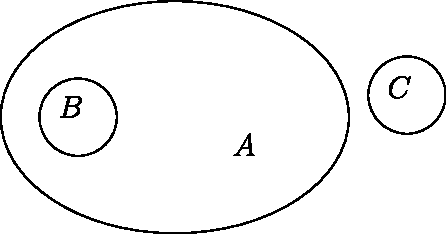
\includegraphics{figures/vennloes1.pdf}
	\end{center}
	2. $A\cap B\not=\emptyset$, $\neg((A\subseteq B)\vee (B\subseteq A)$, $C\subset A$, $C\cap B=\emptyset$
	\begin{center}
		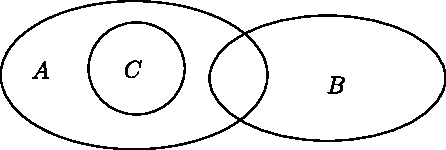
\includegraphics{figures/vennloes2.pdf}
	\end{center}
	3. $B\subset A$, $C\subset B$, $D\subset A$, $D\cap B=\emptyset$
	\begin{center}
		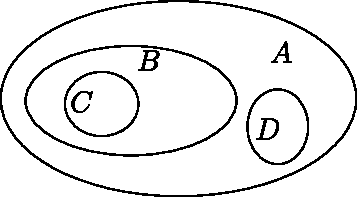
\includegraphics{figures/vennloes3.pdf}
	\end{center}
\end{solution}



\question{{\it Venn-Diagramme -- II}}

\begin{center}
	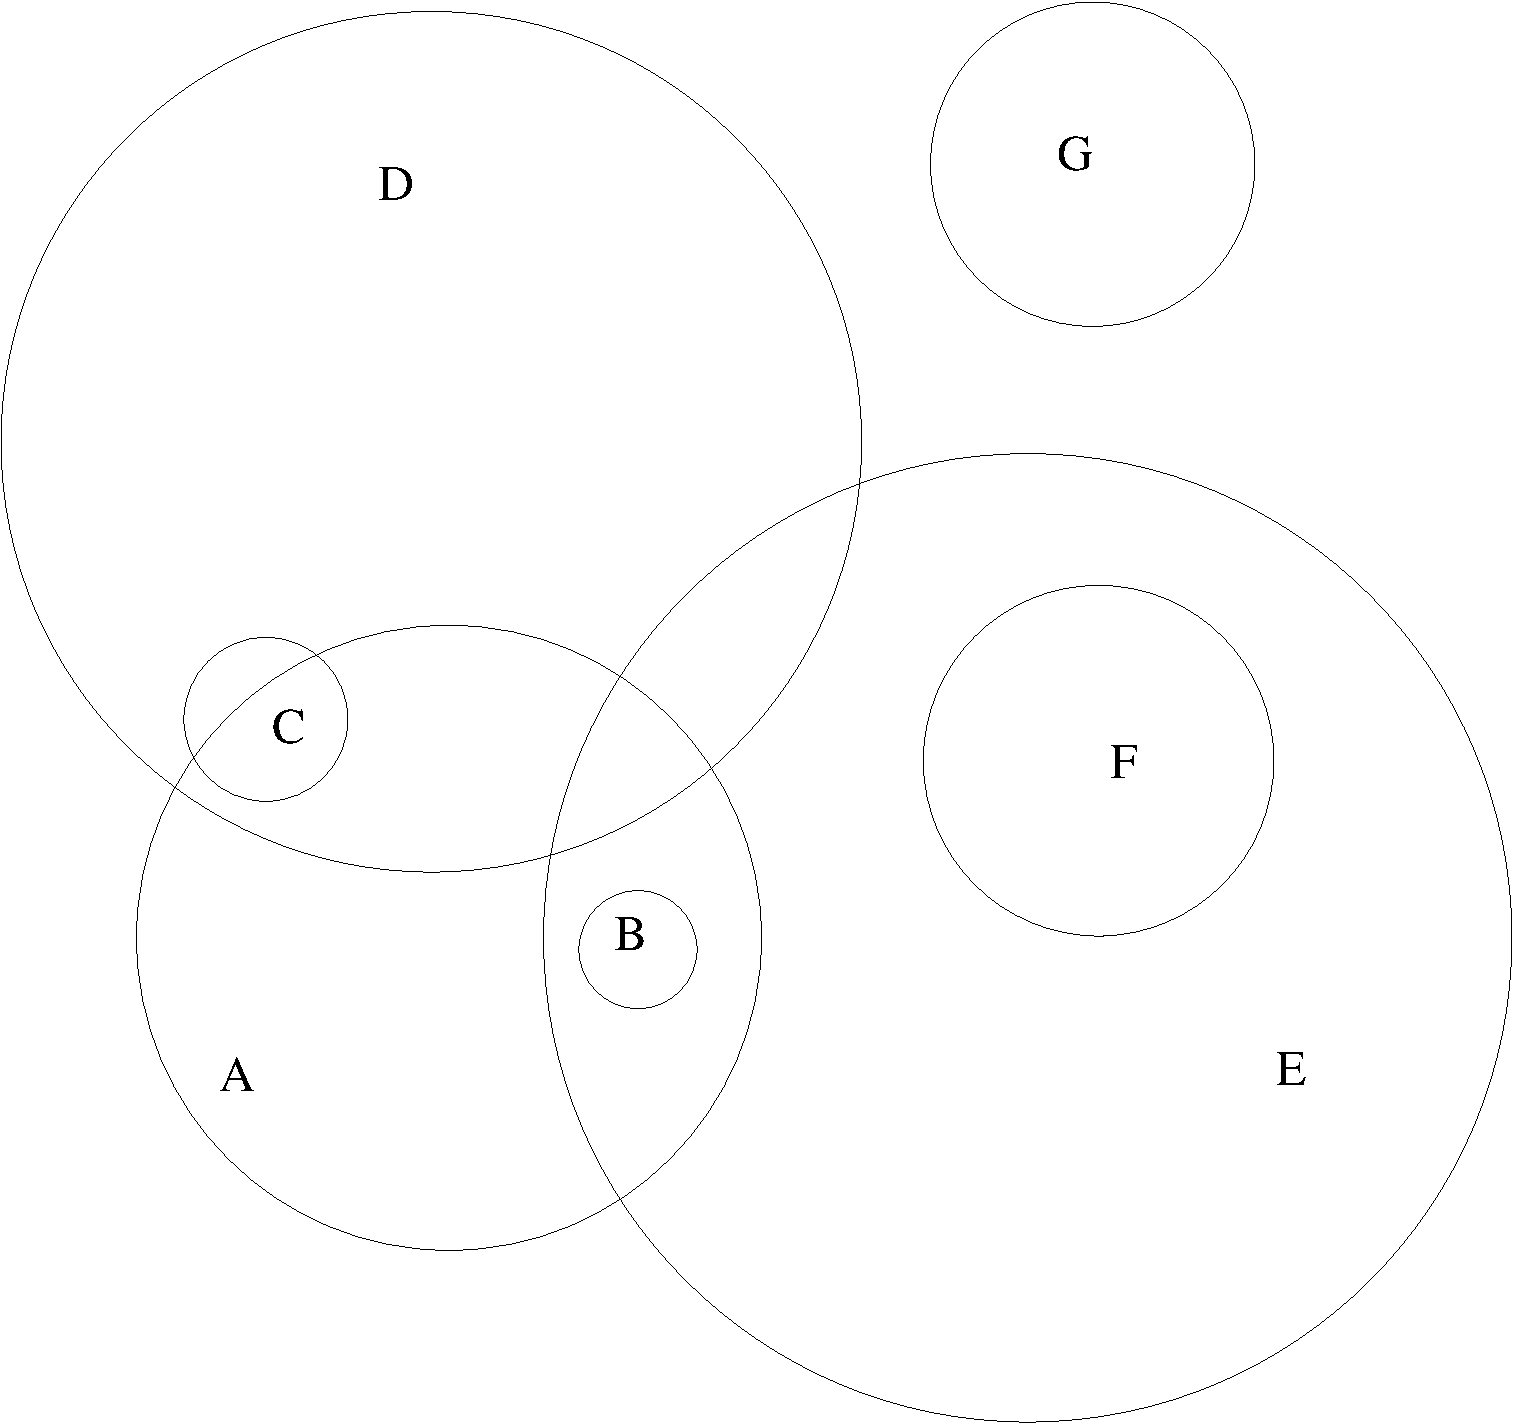
\includegraphics[width=0.65\linewidth,keepaspectratio=]{figures/vennproblemsheet.pdf}
\end{center}

Betrachten Sie das obenstehende Venn-Diagramm, und bestimmen Sie jeweils den Wahrheitswert der folgenden Aussagen:\\
\parbox{0.5\textwidth}{
	\begin{enumerate}
		\item $A\subseteq B$
		\item $B\subset A$
		\item $B\cap C=\emptyset$
		\item $B\subseteq E$
		\item $B\subset(A\cap E)$
		\item $C\subseteq(A\cap D)$
		\item $C\subseteq(A\cup D)$
		\item $F\subset(E\backslash D)$
\end{enumerate}}\parbox{0.5\textwidth}{
	\begin{enumerate}\setcounter{enumi}{8}
		\item $C\subseteq(D\backslash A)$
		\item $C\cap(D\backslash A)=\emptyset$
		\item $F\subset(E\cup G)$
		\item $C\subset(D\backslash E)$
		\item $(C\cap A)\subset D$
		\item $G\cup F=\emptyset$
		\item $F\backslash E=\emptyset$
		\item $(B\cap C)\subseteq (D\cap G)$
\end{enumerate}}
\begin{solution}\\
	\parbox{0.5\textwidth}{
		\begin{enumerate}
			\item falsch
			\item wahr
			\item wahr
			\item wahr
			\item wahr
			\item falsch
			\item wahr
			\item wahr
	\end{enumerate}}\parbox{0.5\textwidth}{
		\begin{enumerate}\setcounter{enumi}{8}
			\item falsch
			\item falsch
			\item wahr
			\item wahr
			\item wahr
			\item falsch
			\item wahr
			\item wahr
	\end{enumerate}}
\end{solution}



\question{{\it Mengentheoretische Gesetze}}

Beweisen Sie folgende Mengentheoretische Gesetze jeweils mit Hilfe des Extensionalitätsprinzips sowie der aussagenlogischen Gesetze aus Aufgabe 1:
\begin{enumerate}
	\item $(A\cap(B\cap C))=((A\cap B)\cap C)$
	\item $(A\cup(B\cup C))=((A\cup B)\cup C)$
	\item $(A\cap(B\cup C))=((A\cap B)\cup(A\cap C))$
	\item $(A\cup(B\cap C))=((A\cup B)\cap(A\cup C))$
\end{enumerate}
\begin{solution}
	\begin{enumerate}
		\item \begin{proof}\begin{align*}
			&x\in(A\cap(B\cap C))\Leftrightarrow x\in A \land x\in (B\cap C) \Leftrightarrow x\in A \land (x\in B \land x\in C)\\
			&\Leftrightarrow(x\in A \land x\in B) \land x\in C \Leftrightarrow x\in((A\cap B)\cap C)
		\end{align*}\end{proof}
		\item \begin{proof}\begin{align*}
			&x\in(A\cup(B\cup C))\Leftrightarrow x\in A \lor x\in (B\cup C) \Leftrightarrow x\in A \lor (x\in B \lor x\in C)\\
			&\Leftrightarrow(x\in A \lor x\in B) \lor x\in C \Leftrightarrow x\in((A\cup B)\cup C)
		\end{align*}\end{proof}
		\item \begin{proof}\begin{align*}
			&x\in(A\cap(B\cup C))\Leftrightarrow x\in A \land x\in (B\cup C) \Leftrightarrow x\in A \land (x\in B \lor x\in C)\\
			&\Leftrightarrow(x\in A \land x\in B) \lor(x\in A \land x\in C) \Leftrightarrow x\in((A\cap B)\cup(A\cap C))
		\end{align*}\end{proof}
		\item \begin{proof}\begin{align*}
			&x\in(A\cup(B\cap C))\Leftrightarrow x\in A \lor x\in (B\cap C) \Leftrightarrow x\in A \lor (x\in B \land x\in C)\\
			&\Leftrightarrow(x\in A \lor x\in B) \land(x\in A \lor x\in C) \Leftrightarrow x\in((A\cup B)\cap(A\cup C))
		\end{align*}\end{proof}
	\end{enumerate}
\end{solution}



\question{{\it Zum Nachdenken und Diskutieren}}

\begin{enumerate}
	\item Machen Sie sich den Unterschied zwischen dem umgangssprachlichen Gebrauch von ``wenn \ldots dann \ldots'' und der Bedeutung des aussagenlogischen $p\Rightarrow q$ an Beispielen wie ``Wenn Du Deine Suppe aufißt, bekommst Du Dessert.'' klar.
	\item Erklären Sie ihrem Banknachbarn Ihre Einsichten.
	\item Wiederholen Sie die beiden vorangehenden Schritte für umgangssprachlichen ``oder'' und aussagenlogisches $\vee$. Welche Unklarheit in der Bedeutung hat das umgangssprachliche ``oder''?
\end{enumerate}


\question{{\it Teilbarkeit und Division mit Rest}}

Bestimmen Sie jeweils, ob eine der beiden angegebenen natürlichen Zahlen die andere teilt. Falls nicht, geben Sie jeweils den Rest bei Division der größeren durch die kleinere Zahl an.\\
\parbox{0.5\textwidth}{\begin{enumerate}
		\item $5$, $15$    %5 teilt 15
		\item $50$, $67$   %67 = 1*50 + 17, Rest 17
		\item $3$, $102$   %3 teilt 102
		\item $129$, $129$   %129 teilt sich selbst
\end{enumerate}}\parbox{0.5\textwidth}{\begin{enumerate}\setcounter{enumi}{4}
		\item $25$, $505$  %505 = 20*25 + 5, Rest 5
		\item $1024$, $9$  %1024 = 113*9 + 7, Rest 7
		\item $10023$, $3$ %3 teilt 10023
		\item $978654321081$, $8$ %8 teilt 1000, also Rest 1
\end{enumerate}}
\begin{solution}\\
	\parbox{0.5\textwidth}{\begin{enumerate}
			\item 5 teilt 15
			\item $67 = 1\cdot50 + 17$, Rest 17
			\item 3 teilt 102
			\item 129 teilt sich selbst
	\end{enumerate}}\parbox{0.5\textwidth}{\begin{enumerate}\setcounter{enumi}{4}
			\item $505 = 20\cdot25 + 5$, Rest 5
			\item $1024 = 113\cdot9 + 7$, Rest 7
			\item 3 teilt 10023
			\item 8 teilt 1000, also Rest 1
	\end{enumerate}}
\end{solution}



\question{{\it Primzahlen und Faktorisierung}}

Bestimmen Sie für die folgenden Zahlen jeweils, ob es sich um Primzahlen handelt. Falls nicht, geben Sie jeweils die Faktorisierung in Primzahlen an.\\
\parbox{0.5\textwidth}{\begin{enumerate}
		\item $3$    %prim
		\item $1$    %nicht prim, 1
		\item $1024$ %nicht prim, 2^10
		\item $243$  %nicht prim, 3^5
\end{enumerate}}\parbox{0.5\textwidth}{\begin{enumerate}\setcounter{enumi}{4}
		\item $3600$ %nicht prim, 2^4 3^2 5^2
		\item $3060$ %nicht prim, 2^2 3^2 5 17
		\item $137$  %prim
		\item $237$  %nicht prim, 3 79
\end{enumerate}}
\begin{solution}
\begin{enumerate}
	\item $3$:    Primzahl
	\item $1$:    Keine Primzahl, Zerlegung nur möglich für $n\in\Nset, n>1$
	\item $1024$: Keine Primzahl (teilbar durch 2)\\Zerlegung: $1024=2^{10}$
	\item $243$:  Keine Primzahl (teilbar durch 3 -- Quersumme)\\Zerlegung: $243=3^5$
	\item $3600$: Keine Primzahl (teilbar durch 2)\\Zerlegung: $3600=2^4\cdot3^2\cdot5^2$
	\item $3060$: Keine Primzahl (teilbar durch 2)\\Zerlegung: $3060=2^2\cdot3^2\cdot5\cdot17$
	\item $137$:  Primzahl
	\item $237$:  Keine Primzahl (teilbar durch 3 -- Quersumme)\\Zerlegung: $237=3\cdot79$
\end{enumerate}
\end{solution}


\pagebreak


\question{{\it Kürzen von Brüchen}}

Kürzen Sie folgende Brüche jeweils soweit wie möglich ($a$, $b$, $c$ seien jeweils beliebige, paarweise teilerfremde, natürliche Zahlen ungleich Null):\\
\parbox{0.5\textwidth}{\begin{enumerate}
		\item $\frac{15}{25}$
		\item $\frac{720a^2}{12ab}$
		\item $\frac{48(a^2-b^2)}{6a+6b}$
		\item $\frac{ab+ac}{(a+b)^2-b^2}$
\end{enumerate}}\parbox{0.5\textwidth}{\begin{enumerate}\setcounter{enumi}{4}
		\item $\frac{(a-b)^3+(b^3-a^3)}{36a}$
		\item $\frac{a^{32}-1024}{a^{16}-32}$
		\item $\frac{a^2+1024}{a+1024}$
		\item $\frac{2310(a^4-b^2)}{4641(a^2+b)}$
\end{enumerate}}
\begin{solution}\\
	\parbox{0.5\textwidth}{\begin{enumerate}
			\item $\frac{3}{5}$
			\item $\frac{60a}{b}$
			\item $8(a-b)$
			\item $\frac{b+c}{a+2b}$
	\end{enumerate}}\parbox{0.5\textwidth}{\begin{enumerate}\setcounter{enumi}{4}
			\item $\frac{b(b-a)}{12}$
			\item $a^{16}+32$
			\item $\frac{a^2+1024}{a+1024}$
			\item $\frac{110}{221}(a^2-b)$
	\end{enumerate}}
\end{solution}


\question{{\it Rechnen mit rationalen Zahlen}}

Formen Sie die folgenden Ausdrücke jeweils so um, dass nur ein soweit wie möglich gekürzter Bruch übrigbleibt:\\
\parbox{0.5\textwidth}{\begin{enumerate}
		\item $\frac{7}{3}+\frac{15}{24}$
		\item $3\cdot\frac{2}{9}-\frac{21+7}{4^2}$
		\item $\frac{4}{7}\cdot\frac{49}{12}$
		\item $\left(2+\frac{1}{137}\right)^3$
\end{enumerate}}\parbox{0.5\textwidth}{\begin{enumerate}\setcounter{enumi}{4}
		\item $\frac{49}{3}-\frac{150-3}{21}$
		\item $\frac{100}{13}\cdot\frac{196}{10}$
		\item $\frac{1+2+3}{2^{10}}\cdot\frac{8^2}{3!}$
		\item $\frac{9}{11}/\frac{121}{27}$
\end{enumerate}}
\begin{solution}\\
	\parbox{0.5\textwidth}{\begin{enumerate}
			\item $\frac{71}{24}$
			\item $-\frac{13}{12}$
			\item $\frac{7}{3}$
			\item $\frac{275^3}{137^3}=\frac{20796875}{2571353}$
	\end{enumerate}}\parbox{0.5\textwidth}{\begin{enumerate}\setcounter{enumi}{4}
			\item $\frac{28}{3}$
			\item $\frac{1960}{13}$
			\item $\frac{1}{16}$
			\item $\frac{3^5}{11^3}=\frac{243}{1331}$
	\end{enumerate}}
\end{solution}



\question{{\it Rationale und Irrationale Zahlen}}

Entscheiden Sie jeweils, ob die folgenden Zahlen rational oder irrational sind, und beweisen Sie gegebenenfalls die Irrationalität:\\
\parbox{0.5\textwidth}{\begin{enumerate}
		\item $\frac{5}{2}$ %rational
		\item $\sqrt{37}$   %irrational, Beweis wie sqrt(2), da 37 prim
		\item $\sqrt{36}$   %=6, rational
\end{enumerate}}\parbox{0.5\textwidth}{\begin{enumerate}\setcounter{enumi}{3}
		\item $\frac{1}{\sqrt{2}}$ %irrational, da sonst rational*irrational=1 sein muesste, im Widerspruch zur Koerpereigenschaft von \Qset
		\item $\frac{1+\sqrt{5}}{2}$ %irrational, da rational+irrational irrational sein muss (sonst Widerspruch zur Koerpereigenschaft von \Qset)
		\item $\frac{(1+\sqrt{5})^2+(1-\sqrt{5})^2}{(1+\sqrt{5})^2-2(1+\sqrt{5})}$ %=12/4=3, rational
\end{enumerate}}
\begin{solution}\\
	\parbox{0.5\textwidth}{\begin{enumerate}
			\item rational
			\item irrational, Beweis wie $\sqrt{2}$, da 37 prim
			\item $\sqrt{36}=6$, rational
	\end{enumerate}}\parbox{0.5\textwidth}{\begin{enumerate}\setcounter{enumi}{3}
			\item irrational, denn angenommen $p/q=1/\sqrt{2}$ ist rational, dann ist auch $q/p=\sqrt{2}$ rational. Widerspruch!
			\item irrational, denn angenommen $p/q=(1+\sqrt{5})/2$ ist rational, dann ist auch $(2p-q)/q=\sqrt{5}$ rational. Widerspruch!
			\item $\frac{(1+\sqrt{5})^2+(1-\sqrt{5})^2}{(1+\sqrt{5})^2-2(1+\sqrt{5})}=12/4=3$, rational
	\end{enumerate}}
\end{solution}



\question{{\it Potenzen und Logarithmen}}

Vereinfachen Sie folgende Ausdrücke jeweils unter Verwendung der Potenz- und Logarithmengesetze soweit, dass höchstens noch eine Potenz oder ein Logarithmus im Ergebnis auftritt ($a,b,c>0$, $n,m\in\Nset$):\\
\parbox{0.5\textwidth}{\begin{enumerate}
		\item $\log_a b + \log_a c -\log_b b^c$
		\item $\log_b a \cdot \log_a b$
		\item $\log_2 1024 - \log_5 125$
		\item $2^{\log_3 9}$
\end{enumerate}}\parbox{0.5\textwidth}{\begin{enumerate}\setcounter{enumi}{4}
		\item $a^n b^n c^{-n}$
		\item $(a^n z^{-n})^{1/(n+1)}$
		\item $a^m a^n$
		\item $(a+b)^m c^m$
\end{enumerate}}
\begin{solution}\\
	\parbox{0.5\textwidth}{\begin{enumerate}
			\item $\log_a (bc) - c$
			\item 1
			\item 7
			\item 4
	\end{enumerate}}\parbox{0.5\textwidth}{\begin{enumerate}\setcounter{enumi}{4}
			\item $\left(\tfrac{ab}{c}\right)^n$
			\item $\left(\tfrac{a}{z}\right)^{n/(n+1)}$
			\item $a^{m+n}$
			\item $(ac+bc)^m$
	\end{enumerate}}
\end{solution}



\question{{\it Wissenschaftliche Notation}}

Schreiben Sie folgende Zahlen jeweils in wissenschaftlicher Notation bzw. als Dezimalbruch:\\
\parbox{0.5\textwidth}{\begin{enumerate}
		\item $0,003$
		\item $1024$
		\item $1\,000\,000\,000$
		\item $0,00000000723455$
\end{enumerate}}\parbox{0.5\textwidth}{\begin{enumerate}\setcounter{enumi}{4}
		\item $1,2\times 10^{-5}$
		\item $9,931\times 10^9$
		\item $7,04\times 10^{-1}$
		\item $1,01\times 10^{3}$
\end{enumerate}}
\begin{solution}\\
	\parbox{0.5\textwidth}{\begin{enumerate}
			\item $3\cdot10^{-3}$
			\item $1,024\cdot10^{3}$
			\item $1\cdot10^{9}$
			\item $7,23455\cdot10^{-9}$
	\end{enumerate}}\parbox{0.5\textwidth}{\begin{enumerate}\setcounter{enumi}{4}
			\item $0,000012$
			\item $9\,931\,000\,000$
			\item $0,704$
			\item $1010$
	\end{enumerate}}
\end{solution}



\question{{\it Komplexe Zahlen}}

Bestimmen Sie für folgende komplexe Zahlen $z$ jeweils Re~$z$, Im~$z$, $|z|$, $\arg(z)$ und $z^*$ ($a$ und $b$ seien jeweils beliebige reelle Zahlen):\\
\parbox{0.5\textwidth}{\begin{enumerate}
		\item $z=a+bi$
		\item $z=4-4i$
		\item $z=13a$
		\item $z=(a^6+5)i$
\end{enumerate}}\parbox{0.5\textwidth}{\begin{enumerate}\setcounter{enumi}{4}
		\item $z=\sqrt{3}-3i$
		\item $z=\sqrt{2}\rme^{\frac{\pi}{4}i}$
		\item $z=\rme^{\frac{\pi}{6}i}$
		\item $z=17\rme^{3\pi i}$
\end{enumerate}}
\begin{solution}
	\begin{enumerate}
		\item $\Re(z)= a, \Im(z)= b, |z|= \sqrt{a^2+b^2}, \arg(z)= \arctan(\tfrac{b}{a})$ für $a>0, z^*= a-bi$
		\item $\Re(z)= 4, \Im(z)= -4, |z|= 4\sqrt{2}, \arg(z)= -\pi/4, z^*= 4+4i$
		\item $\Re(z)= 13a, \Im(z)= 0, |z|= 13a, \arg(z)= 0, z^*= 13a$
		\item $\Re(z)= 0, \Im(z)= a^6+5, |z|= a^6+5, \arg(z)= \pi/2, z^*= -(a^6+5)i$
		\item $\Re(z)= \sqrt{3}, \Im(z)= -3, |z|= 2\sqrt{3}, \arg(z)= -\pi/3, z^*= \sqrt{3}+3i$
		\item $\Re(z)= 1, \Im(z)= 1, |z|= \sqrt{2}, \arg(z)= \pi/4, z^*= \sqrt{2}\rme^{-\frac{\pi}{4}i}$
		\item $\Re(z)= \sqrt{3}/2, \Im(z)= 1/2, |z|= 1, \arg(z)= \pi/6, z^*= \rme^{-\frac{\pi}{6}i}$
		\item $\Re(z)= -17, \Im(z)= 0, |z|= 17, \arg(z)= \pi, z^*= -17$
	\end{enumerate}
\end{solution}



\question{{\it Rechnen mit komplexen Zahlen}}

Formen Sie die folgenden Ausdrücke jeweils in die Form $a+bi$ mit $a,b\in\Rset$ um:\\
\parbox{0.4\textwidth}{\begin{enumerate}
		\item $(3+5i)-(4-2i)$
		\item $\frac{1-2i}{3}+\frac{3+5i}{2}$
		\item $(1+2i)^{-1}$
		\item $(1+i)(1-i)$
		\item $(12+3\sqrt{2}i)\left(\frac{1}{3}-\sqrt{2}i\right)$
		\item $\rme^{\frac{\pi}{2}i}-5\left(2+\rme^{\pi i}\right)$
		\item $\frac{1+i}{1-i}$
\end{enumerate}}\parbox{0.6\textwidth}{\begin{enumerate}\setcounter{enumi}{7}
		\item $\frac{5}{3+4i}$
		\item $(1+i)\rme^{\frac{3\pi}{4}i}$
		\item $\left(\frac{(1+i)^4}{2-2i}\right)^2$
		\item $\left(\rme^{\frac{\pi}{4}i}-1\right)\left(\rme^{\frac{\pi}{4}i}+\frac{1}{2}+\frac{\sqrt{3}}{2}i\right)\left(\rme^{\frac{\pi}{4}i}-\rme^{\frac{2\pi i}{3}}\right)$
		\item $\rme^{\frac{\pi i}{8}}+\rme^{\frac{19\pi i}{24}}+\rme^{-\frac{13\pi i}{24}}$
\end{enumerate}}
\begin{solution}\\
	\parbox{0.4\textwidth}{\begin{enumerate}
			\item $-1+7i$
			\item $\frac{11}{6}+\frac{11}{6}i$
			\item $\frac{1}{5}-\frac{2}{5}i$
			\item $2$
			\item $10-11\sqrt{2}i$
			\item $-5+i$
			\item $i$
	\end{enumerate}}\parbox{0.6\textwidth}{\begin{enumerate}\setcounter{enumi}{7}
			\item $\frac{3}{5}-\frac{4}{5}i$
			\item $-\sqrt{2}$
			\item $2i$
			\item $\left(\rme^{\frac{\pi}{4}i}-1\right)\left(\rme^{\frac{\pi}{4}i}-\rme^{\frac{-2\pi i}{3}}\right)\left(\rme^{\frac{\pi}{4}i}-\rme^{\frac{2\pi i}{3}}\right)\\=\rme^{\frac{3\pi}{4}i}-1=-\frac{1}{\sqrt{2}}-1+\frac{1}{\sqrt{2}}i$
			\item $\rme^{\frac{\pi i}{8}}\left(1+\rme^{\frac{2\pi i}{3}}+\rme^{\frac{-2\pi i}{3}}\right)=0$
	\end{enumerate}}
\end{solution}



\question{{\it Trigonometrische Identitäten}}

Leiten Sie die folgenden trigonometrischen Identitäten jeweils mit Hilfe der Euler-Formel $\rme^{i\alpha}=\cos\alpha+i\sin\alpha$ her:\\
\parbox{0.5\textwidth}{\begin{enumerate}
		\item $\sin(2\alpha)=2\cos\alpha\sin\alpha$
		\item $\cos(3\alpha)=\cos^3\alpha-3\cos\alpha\sin^2\alpha$
		\item $\sin(\alpha+\beta)=\sin\alpha\cos\beta+\sin\beta\cos\alpha$
\end{enumerate}}\parbox{0.5\textwidth}{\begin{enumerate}\setcounter{enumi}{3}
		\item $\cos(\alpha-\beta)=\cos\alpha\cos\beta+\sin\alpha\sin\beta$
		\item $\sin^2(\alpha)=\frac{1}{2}-\frac{1}{2}\cos(2\alpha)$
		\item $\sin(\alpha+\beta)\sin(\alpha-\beta)=\sin^2\alpha-\sin^2\beta$
\end{enumerate}}
\begin{solution}
	\begin{enumerate}
	\item Wir berechnen $\rme^{i\alpha}\cdot \rme^{i\alpha}=\rme^{2i\alpha}$ auf zwei verschiedene Arten und vergleichen daraufhin jeweils Real- und Imaginärteile
	\begin{align*}
		\rme^{2i\alpha}&=\cos(2\alpha)+i\sin(2\alpha)=(\cos(\alpha)+i\sin(\alpha))^2=\cos^2(\alpha)+2i\sin(\alpha)\cos(\alpha)-\sin^2(\alpha)\\
		&\Rightarrow \cos(2\alpha)=\cos^2(\alpha)-\sin^2(\alpha),\\
		&\Rightarrow \sin(2\alpha)=2\sin(\alpha)\cos(\alpha)
	\end{align*}
	\item Analog zu Aufgabe 1 mit $\rme^{i\alpha}\cdot \rme^{i\alpha}\cdot \rme^{i\alpha}=\rme^{3i\alpha}$
	\begin{align*}
		\rme^{3i\alpha}&=\cos(3\alpha)+i\sin(3\alpha)=(\cos(\alpha)+i\sin(\alpha))^3\\
		&=\cos^3(\alpha)+3i\sin(\alpha)\cos^2(\alpha)-3\sin^2(\alpha)\cos(\alpha)-i\sin^3(\alpha)\\
		&\Rightarrow \cos(3\alpha)=\cos^3(\alpha)-3\sin^2(\alpha)\cos(\alpha)
	\end{align*}
	\item Wir berechnen $\rme^{i\alpha}\cdot\rme^{i\beta}=\rme^{i(\alpha+\beta)}$
	\begin{align*}
		&\cos(\alpha+\beta)+i\sin(\alpha+\beta)=(\cos(\alpha)+i\sin(\alpha))\cdot(\cos(\beta)+i\sin(\beta))\\
		&=\cos(\alpha)\cos(\beta)+i(\cos(\alpha)\sin(\beta)+\sin(\alpha)\cos(\beta))-\sin(\alpha)\sin(\beta)\\
		&\Rightarrow\sin(\alpha+\beta)=\cos(\alpha)\sin(\beta)+\sin(\alpha)\cos(\beta)
	\end{align*}
	\item Analog zu Aufgabe 3
	\item Wir verwenden das Resultat $\cos(2\alpha)=\cos^2(\alpha)-\sin^2(\alpha)$ aus Aufgabe 1 und erhalten mit $\sin^2(x)+\cos^2(x)=1$
	\begin{align*}
		\cos(2\alpha)&=1-2\sin^2(\alpha)\\
		&\Rightarrow\sin^2(\alpha)=\frac{1}{2}-\frac{1}{2}\cos(2\alpha)
	\end{align*}
	\item Wir verwenden den Ausdruck aus Aufgabe 3 sowie dessen Transformation für $\beta\rightarrow-\beta$ unter Beachtung von $\sin(-x)=-\sin(x)$ und $\cos(-x)=\cos(x)$
	\begin{align*}
		\sin(\alpha+\beta)\sin(\alpha-\beta)&=(\sin(\alpha)\cos(\beta)+\sin(\beta)\cos(\alpha))(\sin(\alpha)\cos(\beta)-\sin(\beta)\cos(\alpha))\\
		&=\sin^2(\alpha)\cos^2(\beta)-\sin^2(\beta)\cos^2(\alpha)\\
		&=\sin^2(\alpha)(1-\sin^2(\beta))-\sin^2(\beta)\cos^2(\alpha)=\sin^2(\alpha)-\sin^2(\beta)
	\end{align*}
	\end{enumerate}
\end{solution}





\question{{\it Beweis mittels vollständiger Induktion}}

Beweisen Sie folgenden Aussagen jeweils mittels vollständiger Induktion:\\
\parbox{0.5\textwidth}{\begin{enumerate}
		\item $\forall n\in\Nset~n^2=\sum\limits_{k=0}^{n-1} (2k+1)$
		\item $\forall n\in\Nset~ 2^n-1=\sum\limits_{k=0}^{n-1} 2^k$
		\item $\forall n\in\Nset~\sum\limits_{k=0}^{n-1} 3^k = \frac{3^n-1}{2}$ 
\end{enumerate}}\parbox{0.5\textwidth}{\begin{enumerate}\setcounter{enumi}{3}
		\item $\forall n\in\Nset~\sum\limits_{k=0}^n k=\frac{n(n+1)}{2}$ 
		\item $\forall n\in\Nset~\sum\limits_{k=0}^{n-1} (2k+1)^2=\frac{n(2n-1)(2n+1)}{3}$
		\item $\forall n\in\Nset~\forall x\in[0;\infty)~(1+x)^n\ge 1+nx$
\end{enumerate}}
\begin{solution}
	Sei $n_0$ eine ganze Zahl und $A(n)$ für jede ganze Zahl $n\geq n_0$ eine Aussage. Um $A(n)$ für alle $n\geq n_0$ zu beweisen, genügt es zu zeigen, dass
	\begin{enumerate}
		\item[(IA)] $A(n_0)$ ist richtig (Induktions-Anfang).
		\item[(IS)] Für ein beliebiges $n\geq n_0$ gilt: Falls $A(n)$ richtig ist, so ist auch $A(n+1)$ richtig (Induktions-Schritt).
	\end{enumerate}
	\begin{enumerate}
		\item \begin{proof}
			(IA) $n_0=1$: $1^2=0+1$\checkmark. Nun betrachten wir $n\geq n_0$ und nehmen an, dass die Behauptung gilt. Dann ist
			\[(n+1)^2=n^2+2n+1=\sum\limits_{k=0}^{n-1} (2k+1)+(2n+1)=\sum\limits_{k=0}^{(n+1)-1} (2k+1)
			\]
		\end{proof}
		\item \begin{proof}
			(IA) $n_0=1$: $2-1=2^0$\checkmark. Nun betrachten wir $n\geq n_0$ und nehmen an, dass die Behauptung gilt. Dann ist
			\[2^{n+1}-1=2(2^n-1)+1=2\sum\limits_{k=0}^{n-1} 2^k+1=\sum\limits_{k=1}^{n} 2^k+1=\sum\limits_{k=0}^{(n+1)-1} 2^k
			\]
		\end{proof}
		\item \begin{proof}
			(IA) $n_0=1$: $3^0=\frac{3^1-1}{2}$\checkmark. Nun betrachten wir $n\geq n_0$ und nehmen an, dass die Behauptung gilt. Dann ist
			\[\sum\limits_{k=0}^{n} 3^k = \sum\limits_{k=0}^{n-1}3^k+3^n= \frac{3^n-1}{2}+3^n=\frac{2\cdot 3^n+3^n-1}{2}=\frac{3^{n+1}-1}{2}
			\]
		\end{proof}
		\item {\it Hinweis:} Hierbei handelt es sich um die Gaußsche Summenformel
		\begin{proof}
			(IA) $n_0=1$: $0+1=\frac{1\cdot2}{2}$\checkmark. Nun betrachten wir $n\geq n_0$ und nehmen an, dass die Behauptung gilt. Dann ist
			\[\sum\limits_{k=0}^{n+1} k=\sum\limits_{k=0}^{n}k+n+1=\frac{n(n+1)}{2}+n+1=\frac{n(n+1)+2(n+1)}{2}=\frac{(n+1)(n+2)}{2}
			\]
		\end{proof}
		\item \begin{proof}
			(IA) $n_0=1$: $(0+1)^2=\frac{1\cdot1\cdot3}{3}$\checkmark. Nun betrachten wir $n\geq n_0$ und nehmen an, dass die Behauptung gilt. Dann ist
			\begin{align*}
				\sum\limits_{k=0}^{n} (2k+1)^2&=\sum\limits_{k=0}^{n-1} (2k+1)^2+(2n+1)^2=\frac{n(2n-1)(2n+1)}{3}+(2n+1)^2\\
				&=\frac{n(2n-1)(2n+1)+3(2n+1)^2}{3}=\frac{(n+1)(2n+1)(2n+3)}{3}
			\end{align*}
		\end{proof}
		\item \begin{proof}
			(IA) $n_0=1$: $1+x\geq 1+x$\checkmark. Nun betrachten wir $n\geq n_0$ und nehmen an, dass die Behauptung gilt. Dann ist
			\[(1+x)^{n+1}=(1+x)(1+x)^n\ge (1+x)(1+nx)=1+x+nx+nx^2\geq 1+(n+1)x
			\]
		\end{proof}
	\end{enumerate}
\end{solution}


\question{{\it Polynomdivision}}

Führen Sie für die folgenden Paare von Polynomen jeweils die Polynomdivision durch.
\begin{enumerate}
	\item $(x^3-x^2-5x-3)$, $(3-x)$
	\item $(x^4+3x^3+4x^2+3x+1)$, $(x^2+x+1)$
	\item $(6 x^4-12 x^3+37 x^2-48 x+45)$, $(2 x^2-4 x+4)$
	\item $(x^5+4 x^4-9 x^3-40 x^2-4 x+48)$, $(x^2+4x+4)$
	\item $(x^5+4 x^4-9 x^3-40 x^2-4 x+48)$, $(x^3-13 x+12)$
	\item $(2 x^8+4 x^7+3 x^6-5 x^5-16 x^4-13 x^3+4 x^2-4 x+18)$, $(x^3+x-4)$
	\item $(x^8-4 x^7+14 x^6-4 x^5+13 x^4+x^2-3)$, $(x^5-4 x^4+13 x^3)$
	\item $(x^{10}-1)$, $(1 - x + x^2 - x^3 + x^4)$
\end{enumerate}
\begin{solution}
	\begin{enumerate}
		\item \polylongdiv[style=C]{x^3-x^2-5x-3}{3-x}\\
		\item $x^2+2x+1$
		\item $3x^2+\frac{25}{2}+\frac{2x-5}{2 x^2-4 x+4}$
		\item $x^3-13x+12$
		\item $x^2+4x+4$
		\item $2x^5+4x^4+x^3-x^2-x-8+\frac{x^2-14}{x^3+x-4}$
		\item $x^3+x+\frac{x^2-3}{x^5-4 x^4+13 x^3}$
		\item $x^6+x^5-x-1$
	\end{enumerate}
\end{solution}



\question{{\it Faktorisierung von Polynomen}}

Bestimmen Sie für die folgenden Polynome jeweils alle reellen Nullstellen und überprüfen Sie, ob das Polynom über $\Rset$ in Linearfaktoren zerfällt. Falls nicht, geben Sie die verbleibenden quadratischen Faktoren an und bestimmen Sie die zugehörigen komplexen Nullstellen.\\
\parbox{0.5\textwidth}{\begin{enumerate}
		\item $x^2-2x+1$
		\item $x^2+2x+1$ 
		\item $x^2+4$
		\item $x^3+9x$
\end{enumerate}}\parbox{0.5\textwidth}{\begin{enumerate}\setcounter{enumi}{4}
		\item $x^3-13 x+12$
		\item $x^3-5 x^2+7 x-3$
		\item $6 x^4-12 x^3+36 x^2-48 x+48$ 
		\item $x^8 - 2 x^4 + 1$
\end{enumerate}}
\begin{solution}
	Im Folgenden bezeichnet $\mathcal{N}\subset\Rset$ die Menge der reellen Nullstellen der jeweiligen Polynome
	\begin{enumerate}
		\item $\mathcal{N}=\{1\}, (x-1)^2$
		\item $\mathcal{N}=\{-1\}, (x+1)^2$
		\item $\mathcal{N}=\emptyset, (x-2i)(x+2i)$
		\item $\mathcal{N}=\{0\}, x(x-3i)(x+3i)$
		\item $\mathcal{N}=\{-4, 1, 3\}, (x-3)(x-1)(x+4)$
		\item $\mathcal{N}=\{1, 3\}, (x-3)(x-1)^2$
		\item $\mathcal{N}=\emptyset, 6(x+2i)(x-2i)(x-1+i)(x-1-i)$
		\item $\mathcal{N}=\{-1, 1\}, (x+1)^2(x-1)^2(x+i)^2(x-i)^2$
	\end{enumerate}
\end{solution}

\pagebreak




\end{questions}

\end{document}
